%\documentclass[mathserif]{beamer}
\documentclass[handout]{beamer}
%\usetheme{Goettingen}
\usetheme{Warsaw}
%\usetheme{Singapore}
%\usetheme{Frankfurt}
%\usetheme{Copenhagen}
%\usetheme{Szeged}
%\usetheme{Montpellier}
%\usetheme{CambridgeUS}
%\usecolortheme{}
%\setbeamercovered{transparent}
\usepackage[english, activeacute]{babel}
\usepackage[utf8]{inputenc}
\usepackage{amsmath, amssymb}
\usepackage{dsfont}
\usepackage{graphics}
\usepackage{cases}
\usepackage{graphicx}
\usepackage{pgf}
\usepackage{epsfig}
\usepackage{amssymb}
\usepackage{multirow}	
\usepackage{amstext}
\usepackage[ruled,vlined,lined]{algorithm2e}
\usepackage{amsmath}
\usepackage{epic}
\usepackage{fontenc}
\usepackage{framed,color}
\usepackage{palatino, url, multicol}
\usepackage{listings}
%\algsetup{indent=2em}
\vspace{-0.5cm}
\title{Design of Experiments \& Hypothesis Testing}
\vspace{-0.5cm}
\author[Felipe Bravo Márquez]{\footnotesize
%\author{\footnotesize  
 \textcolor[rgb]{0.00,0.00,1.00}{Felipe José Bravo Márquez}} 
\date{ \today }






\begin{document}
\begin{frame}
\titlepage


\end{frame}


%%%%%%%%%%%%%%%%%%%%%%%%%%%

% Useful references: http://www.buders.com/UNIVERSITE/Universite_Dersleri/istatistik/sampling_distributions_and_point_estimation_of_parameters.pdf
% http://homepage.divms.uiowa.edu/~rdecook/stat2020/notes/ch7_pt1.pdf


\begin{frame}{Motivation}
\scriptsize{


In the first lecture we discussed the three major goals of statistics:
\begin{enumerate}
 \item Describe
 \item Decide
 \item Predict 
\end{enumerate}



 \begin{itemize}
  \item In this lecture we will introduce the ideas behind the use of statistics to make decisions.
  \item In particular, decisions about whether a particular \textbf{hypothesis} is supported by the data. \cite{poldrack2019statistical}
 \end{itemize}

} 
\end{frame}



\begin{frame}{Null Hypothesis Statistical Testing (NHST)}
\scriptsize{
\begin{itemize}
 \item The specific type of hypothesis testing that we will discuss is known null hypothesis statistical testing (NHST).
\item  If you pick up almost any scientific research publication, you will see NHST being used to test hypotheses.
\item Learning how to use and interpret the results from hypothesis testing is essential to understand the results from many fields of research.
\item NHST is usually applied to \textbf{experimental} data.
\item Thus, we need to introduce basic concepts on the design of experiments.
\end{itemize}



} 
\end{frame}

\section{Experiments}

\begin{frame}{Experiments and Inference About Cause}
\scriptsize{
\begin{itemize}
 \item In the previous lecture we studied how to infer characteristics of a population from sample data using surveys or polls.
 \item A second type of inference is when we want to infer \textbf{cause-effect relationships} between two or more variables (e.g, does smoking cause cancer) from experimental data. 
 \item Example \cite{watkins2010statistics}: Children who drink more milk have bigger feet than children who drink less milk. 
 
 
\end{itemize}


\begin{figure}[h!]
	\centering
	
\includegraphics[scale=0.25]{pics/milk.png}
	\caption{Image source: \url{https://www.dreamstime.com}}
\end{figure}



} 
\end{frame}


\begin{frame}{Experiments and Inference About Cause}
\scriptsize{

\begin{itemize}
\item There are three possible explanations for this association:
 \begin{enumerate}
 \scriptsize{
 \item Drinking more milk causes children’s feet to be bigger.\\
	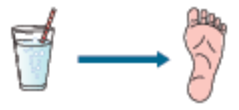
\includegraphics[scale=0.25]{pics/cause1.png}

 
 \item Having bigger feet causes children to drink more milk. \\
 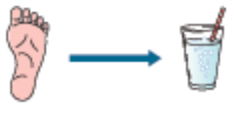
\includegraphics[scale=0.25]{pics/cause2.png}
 
 \item A \textbf{lurking variable} is responsible for both. \\
 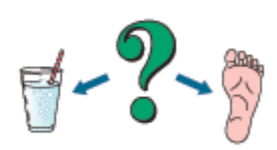
\includegraphics[scale=0.25]{pics/cause3.png}
 }
\end{enumerate}


 \item A lurking variable is a variable that may or may not be apparent at the outset but, once identified, could explain the pattern between the variables.

\item We know that bigger children have bigger feet, and they drink more milk because they eat and drink more of everything than do smaller children.


\end{itemize}



} 
\end{frame}



\begin{frame}{Experiments and Inference About Cause}
\scriptsize{

\begin{itemize}

\item The right explanation is the third one: the child's \textbf{overall size} is the lurking variable.

 \item However, suppose we want to prove that explanation 1 is the right reason with the following approaches. 
 \item Approach 1: take a bunch of children, give them milk, and wait to see if their feet grow.
 \item This won't prove anything, because children's feet will grow whether they drink milk or not.
 \item Approach 2: take a group of children, divide them randomly into two \textbf{groups}: 1) one group that will drink milk and 2) another group that will not, wait and compare the size of the feet of both groups. 
 \item This approach is an \textbf{experiment}, and is the only way to establish cause and effect.
 
\end{itemize}



} 
\end{frame}


\begin{frame}{Main Concepts of Experimental Design}
\scriptsize{


\begin{itemize}
 \item \textbf{Experimental units}: the subjects on which we experiment (e.g, patients, users, laboratory animals). When the experiment units are people, we call them  \textbf{subjects}.
 \item \textbf{Treatments}: the conditions on which we compare different unit groups. Examples: drinking milk vs. not drinking milk, smoking vs. not smoking, taking drug A vs. drug B.
 \item \textbf{Treatment or Experimental group}: a group of units receiving a particular treatment. Example: patients taking a new drug, software users seeing a new layout.
 \item \textbf{Control group}: a group of units used for comparison receiving either a standard treatment or no treatment at all. Example: patients taking a placebo (a fake treatment), software users seeing the standard layout.
 
  \item \textbf{Response variable}: the variable of interest used to measure the effect of the treatments on the units. Examples: weight, birth rate, antibody levels, click-rate, revenue, etc.
 
\end{itemize}



} 
\end{frame}


\begin{frame}{Main Concepts of Experimental Design}
\scriptsize{


\begin{itemize}

 \item \textbf{Randomization}: random assignment of treatments (including the control group) to units. This is very important since not all units are alike (e.g., people have different ages, weights, preferences). \\
 \begin{itemize}
 \scriptsize{
  \item  Randomization is the most reliable method of creating homogeneous treatment groups, without involving any potential biases or judgments.
 }
 \end{itemize}


  \item \textbf{Replication}: the repetition of an experiment on a large group of subjects. Replication reduces variability in experimental results. 
  
  \item \textbf{Randomized Controlled Trial} (RCT): an experiment in which units are randomly assigned to one of several treatments and one of these groups is a control group.
  
  \item \textbf{Blind Experiment}:  when the units (e.g., patients) don't know the treatment they are receiving.
  
  \item \textbf{Double-blind Experiment}: when neither the units (e.g., patients) nor the experimenters (e.g., doctors) know who is receiving a particular treatment.
  
\end{itemize}



} 
\end{frame}


\begin{frame}{Main Concepts of Experimental Design}
\scriptsize{

\begin{figure}[h!]
	\centering
	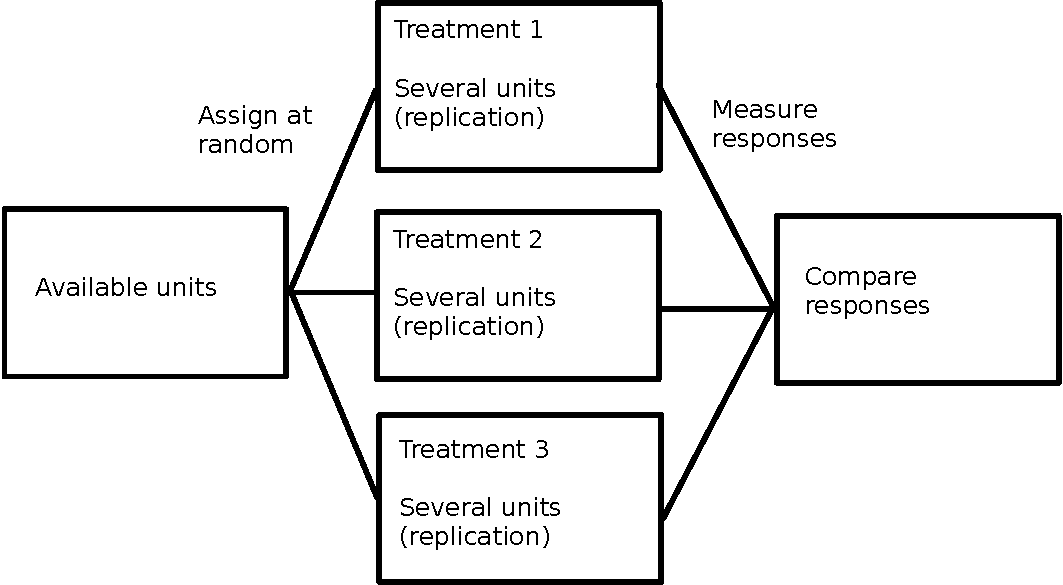
\includegraphics[scale=0.6]{pics/experiment.pdf}
\end{figure}

Characteristics of a well-designed experiment.


} 
\end{frame}


\begin{frame}{A/B Testing}
\scriptsize{


\begin{itemize}

\item Data-driven companies like Amazon, Microsoft, eBay, Facebook, Google and Netflix constantly conduct experiments to make decisions \cite{kohavi2012trustworthy}.

\item In this context, experiments are called \textbf{online  controlled experiments} or \textbf{A/B tests}. 
 

 \item The idea is the same, users (experimental units) are randomly exposed to one of two variants of the software: Control (A), or Treatment (B).
 
 \item When there is more than one treatment we have an A/B/n test.
 
 \item The response variable is called \textbf{Overall  Evaluation  Criterion} (OEC), which is a quantitative measure of the experiment's objective. 
 
 \item OECs can be revenue, clickthrough-rate, user session duration, etc...
 \end{itemize}

} 
\end{frame}


\begin{frame}{A/B Testing}

 \begin{figure}[h!]
	\centering
	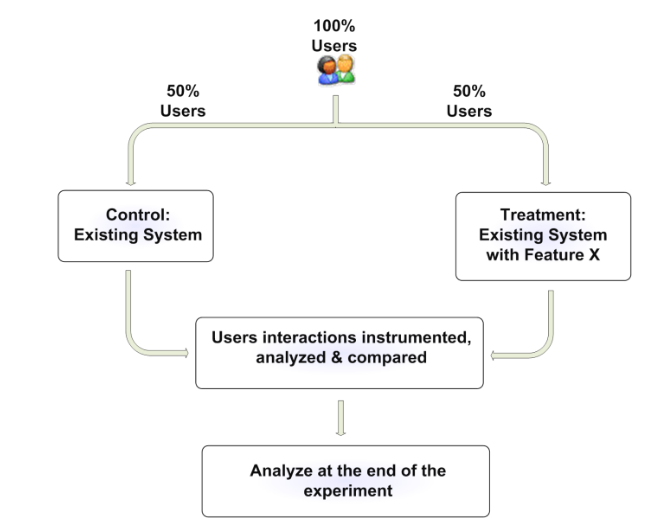
\includegraphics[scale=0.34]{pics/abtest.png}
\end{figure}
Image source: \cite{kohavi2012trustworthy} 
\end{frame}



\begin{frame}{Example: MSN Real Estate}
\scriptsize{


\begin{itemize}

\item The team running the MSN Real Estate site wanted to test different designs for the ``Find a home'' widget \cite{kohavi2009online}.

\item Visitors who click on this widget are sent to partner sites, and Microsoft receives a referral fee. 

\item Six different designs of this widget, including the incumbent (control), were proposed.

\item Users were randomly splited between the variants in a persistent manner (a user receives the same experience in multiple visits) during the experiment period.

\end{itemize}



} 
\end{frame}


\begin{frame}{Example: MSN Real Estate}


\begin{figure}[h!]
	\centering
	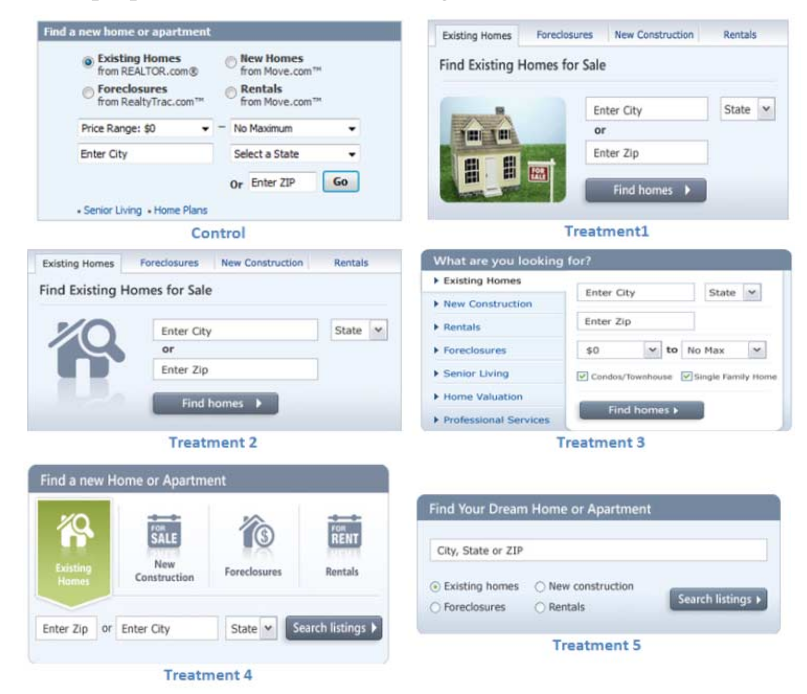
\includegraphics[scale=0.4]{pics/widgets.png}
\end{figure}




\end{frame}


\begin{frame}{Example: MSN Real Estate}
\scriptsize{


\begin{itemize}


 
 \item Their interactions are instrumented and key metrics computed. 
 
 \item In this experiment, the Overall Evaluation Criterion (OEC) was average revenue per user.
 \item The winner, Treatment 5, increased revenues by almost 10\% (due to increased clickthrough).
 
 \item The Return-On-Investment (ROI) for MSN Real Estate was phenomenal, as this is their main source of revenue, which increased significantly through a simple change.

\end{itemize}



} 
\end{frame}




\begin{frame}{Observational Studies and Confounding}
\scriptsize{

\begin{itemize}

 \item Sometimes we can't randomly assign units to the different treatments.
 
 \item For example, it would be unethical to design a randomized controlled trial deliberately exposing people to a potentially harmful situation. 
 
 \item In an \textbf{observational study} the conditions of interest are already built into the units being studied.
 
 \item Observational studies are almost always worse than controlled experiments for determining cause-effect relationships.
 
 \item But sometimes is the only thing we can do.
 
 \item A phenomenon called \textbf{confounding} is the major treat to observational studies.
 
 \item Two possible influences on an observed outcome are \textbf{confounded} if they are mixed in a way that makes it impossible to separate their effects on the responses \cite{watkins2010statistics}.
  
\end{itemize}



} 
\end{frame}

\begin{frame}{A Confounded Observational Study}
\scriptsize{

\begin{itemize}

 \item The thymus, a gland in your neck, behaves in a peculiar way. 
 
 \item Unlike other organs of the body, it doesn't get larger as you grow—it actually gets smaller. 
 \item Ignorance of this fact led early 20th-century surgeons to adopt a worthless and dangerous surgical procedure.
 
 \begin{figure}[h!]
	\centering
	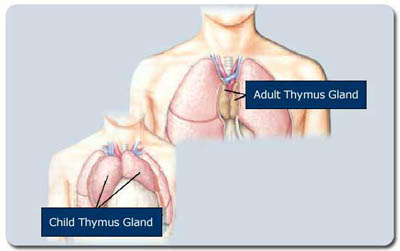
\includegraphics[scale=0.4]{pics/ThymusSizeDiagram.jpg}
	\caption{source: \url{http://esvc001414.wic005tu.server-web.com/tech_imm_bio_principle.htm}}
\end{figure}
 
  
\end{itemize}



} 
\end{frame}


\begin{frame}{A Confounded Observational Study}
\scriptsize{

\begin{itemize}

 \item Many infants were dying of what seemed to be respiratory obstructions.
 
 \item Doctors did autopsies on infants who died with respiratory symptoms and compared against autopsies made on adults who died of various causes.

\item Most autopsies to infants show big thymus glands compared to adults.

\item Doctors concluded that the respiratory problems were caused by an enlarged thymus. 


\item In 1912, Dr. Charles Mayo published an article recommending removal of the thymus to treat respiratory problems in children. 

\item This recommendation was made even though a third of the
children who were operated on died. 
  
\item The doctors could not tell whether children with a large thymus tended to have more respiratory problems because they had no evidence about children with a smaller thymus.  
  
\end{itemize}



} 
\end{frame}



\begin{frame}{A Confounded Observational Study}
\scriptsize{

\begin{itemize}


\item Age and size of thymus were confounded.

\item The thymus study is an example of an observational study, not an experiment.

\begin{table}
\center
 \begin{tabular}{|c|ccc|}  \hline
 
& & \multicolumn{2}{c|}{Age} \\ \hline
& & Child & Adult \\
\multirow{2}{*}{ Thymus size } & Large & Problems & No evidence \\ 
& Small & No evidence & No problems \\ \hline
\end{tabular} 
\end{table}

\item If Dr. Mayo had used a randomized experiment to evaluate surgical removal of the thymus, he would have seen that the treatment was not effective and many lives might have been
spared. 
\item However, at the time, randomized experiments were not often used in the medical profession.
  
\item These days, any new medical treatment (e.g., a COVID vaccine) must prove its value in an RCT.  
\end{itemize}



} 
\end{frame}

\begin{frame}{Another Example of Confounding}
\scriptsize{

\begin{itemize}

\item Suppose we want to compare student performance on a standardized tests (e.g., SIMCE, PSU) between public and private schools.

\item We know that the socioeconomic distribution of students is different in public and private schools.

\item We also suspect that socioeconomic background may influence student performance on these tests.

\item The type of school (public or private) and the socioeconomic background are confounded.
  
\end{itemize}



} 
\end{frame}



\begin{frame}{Randomized Paired Comparison (Matched Pairs)}
\scriptsize{

\begin{itemize}

\item Randomized Paired Comparison or Matched Pairs is an approach to design experiments \textbf{controlling} for confounding variables. 

\item We sort the experimental units into pairs of similar units (matched pairs or \textbf{blocks}), where similarity is measured according to confounding variables.

\item  The two units in each pair should be enough alike that you expect them to have a similar response to any treatment.

\item Randomly decide which unit in each pair is assigned which treatment.

\item We are essentially building comparable Control and Treatment populations by segmenting the users by common confounds, similarly to stratified sampling.
  
\end{itemize}



} 
\end{frame}


\begin{frame}{Matched Pairs Example}
\scriptsize{

\begin{itemize}

\item Suppose we want to study the relation between hypertension and end-stage renal disease (ESRD) \cite{de2011matching}.

\item Obesity is a potential confounder as obesity is associated with both hypertension and ESRD. 

\item Matching approach: we ensure that the average body mass index (BMI) is the same in the group of patients exposed to hypertension and another group of patients unexposed to hypertension. 

\item This could be achieved by searching an obese patient without hypertension for each obese patient with hypertension.
  
\item Other potential confounding variables like age or sex could also be considered in the matching.  
  
\end{itemize}



} 
\end{frame}


\section{Hypothesis Testing}

\begin{frame}{Hypothesis Testing}
\scriptsize{
\begin{itemize}
 \item Now that we understand what experimental data looks like we are in place to introduce  Null Hypothesis Statistical Testing (NHST).
  \item A \textbf{hypothesis test} allows us to  to measure whether some assumed \textbf{property} about a population is contrasted with a statistical sample.
 \item In the context of experiments, NHST helps us to determine weather observed differences between treatment and control groups are unlikely to have occurred by chance. 
 
  \item Hypothesis testing can be applied to all kinds of population parameters (e.g., mean, variance, median).
 \item In the class we will focus on testing the \textbf{population mean} $\mu$.

\end{itemize}
} 
\end{frame}


\begin{frame}{Hypothesis Testing}
 \scriptsize{

\begin{itemize}

 \item We will study the following types of parametric tests to the mean:
 \begin{enumerate}
 \scriptsize{
  \item \textbf{One sample test}: we contrast the sample mean to a pre-specified value.
  \item \textbf{Unpaired two sample test}: we compare the sample means of two independent groups (control vs. treatment).
  \item \textbf{Paired two sample test}: here we compare the means of two dependent groups where we have two values for the same samples. For example: in matched pairs experiments.}
 \end{enumerate}

  \item All these tests can be one-sided or two-sided.
  
  \item In the same way as for confidence intervals we will use Normal and T-student distributions for modeling the sampling distribution of sample means.
  
   \item Warning: there are many counterintuitive concepts around NHST (e.g., null hypothesis, p-values).
 \item Thus, we will fist introduce these concepts with two  examples taken from \cite{poldrack2019statistical} and \cite{Marchini}.
 \item Then we will formalize them in more detail.
  

\end{itemize}

}

%\item Unpaired two sample t-test: better using \url{https://en.wikipedia.org/wiki/Welch\%27s_t-test}
% \item Paired two sample t-test
%\url{https://www.datanovia.com/en/lessons/types-of-t-test/\#one-sample-t-test}
%\url{https://en.wikipedia.org/wiki/Student\%27s_t-test}
% Nice explanations of degrees of freedom: \url{https://crumplab.github.io/statistics/t-tests.html}
%https://stats.stackexchange.com/questions/342074/hypothesis-testing-null-hypothesis-for-one-sided-tests
\end{frame}


\begin{frame}{Example 1: Body-worn Cameras}
\scriptsize{
\begin{itemize}
 \item Body-worn cameras are thought to reduce the use of force and improve behavior of police officers. 

 \item An  RCT of the effectiveness of body-worn cameras was performed by the Washington, DC government and DC Metropolitan Police Department in 2015/2016.
 \item Officers were randomly assigned to wear a body-worn camera or not.
 \item Their behavior was then tracked over time to determine whether the cameras resulted in less use of force and fewer civilian complaints about officer behavior.
 \end{itemize}

 \begin{figure}[h!]
	\centering
	
\includegraphics[scale=0.25]{pics/camera.png}
	\caption{source: \url{https://www.nytimes.com}}
\end{figure}

} 
\end{frame}


\begin{frame}{Example 1: Body-worn Cameras}
\scriptsize{
\begin{itemize}
 \item Let's say we want to specifically test the hypothesis of whether the use of force is decreased by the wearing of cameras. 
 \item The RCT provides us with the data to test the hypothesis – namely, the rates of use of force by officers assigned to either the camera or control groups. 
 \item The next obvious step is to look at the data and determine whether they provide convincing evidence for or against this hypothesis. 
 \item That is: What is the likelihood that body-worn cameras reduce the use of force, given the data and everything else we know?
\item It turns out that this is \textbf{not} how null hypothesis testing works. 

\end{itemize}


} 
\end{frame}


\begin{frame}{Example 1: Body-worn Cameras}
\scriptsize{
\begin{itemize}
\item Instead, we first take our hypothesis of interest (i.e. that body-worn cameras reduce use of force), and flip it on its head, creating a \textbf{null hypothesis}.
\item In this case, the null hypothesis would be that cameras do not reduce use of force. 
\item Importantly, we then assume that the null hypothesis is true. 
\item We then look at the data and determine how likely the data would be if the null hypothesis were true. 
\item If the data are sufficiently unlikely under the null hypothesis that we can reject the null in favor of the \textbf{alternative hypothesis} which is our hypothesis of interest. 
\item If there is not sufficient evidence to reject the null, then we say that we retain (or ``fail to reject'') the null.

\item Then we stick with our initial assumption that the null is true.
 
\end{itemize}


} 
\end{frame}



\begin{frame}{Example 2: Babies}
\scriptsize{
\begin{itemize}
  \item From previous experience we know that the birth weights of babies in England have a mean of 3000g and a standard deviation of 500g.
 \item We think that maybe babies in Australia have a mean birth weight greater than 3000g and we would like to test this hypothesis.
  \item We take a sample of babies from Australia, measure their birth weights and see if the sample mean is significantly larger than 3000g. 
    \item The main hypothesis that we are most interested in is the \textbf{research hypothesis}, denoted $H_1$, that the mean birth weight of Australian babies is greater than 3000g.
\end{itemize}


} 
\end{frame}

\begin{frame}{Example 2: Babies}
\scriptsize{
\begin{itemize}

  \item The other hypothesis is the null hypothesis, denoted $H_0$, that the mean birth weight is equal to 3000g.
\item We can write this compactly as:
\begin{table}
\center
 \begin{tabular}{c}  
$H_0$: $\mu=3000g$ \\
$H_1$: $\mu>3000g$
\end{tabular} 
\end{table}

\item The null hypothesis is written first followed by the research hypothesis. 
\item The research hypothesis is often called the \textbf{alternative hypothesis} even though it is often the first hypothesis we think of.

\end{itemize}


} 
\end{frame}


\begin{frame}[fragile]{Example 2: Babies}
\scriptsize{
\begin{itemize}
  \item Normally, we start with the research hypothesis and ``set up'' the null hypothesis to be directly counter to what we hope to show. 
  \item We then try to show that, in the light of our collected data, that the null hypothesis is false. 
  \item We do this by calculating the probability of the data if the null hypothesis is true. 
  \item If this probability is very small, it suggests that the null hypothesis is false.
  \item Once we have set up our null and alternative hypothesis, we can collect a sample of data. 
  \item For example, we can imagine we collected the birth weights of the 44 babies in the Babyboom dataset.

\end{itemize}
\begin{verbatim}
>library(UsingR)
>data(babyboom)
>hist(babyboom$wt)
\end{verbatim}


} 
\end{frame}


\begin{frame}[fragile]{Example 2: Babies}
\scriptsize{

 \begin{figure}[h!]
	\centering
	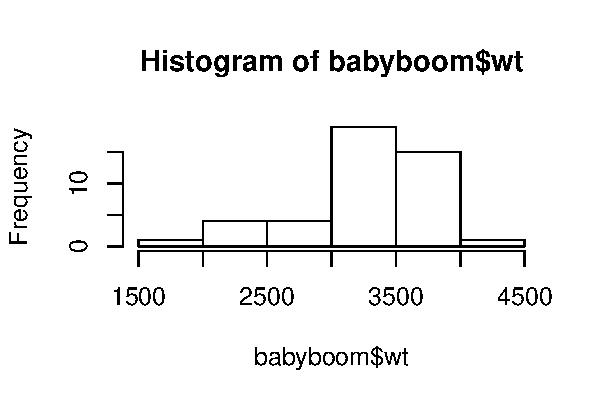
\includegraphics[scale=0.6]{pics/babyhist.pdf}
\end{figure}

\begin{itemize}
 \item The sample mean of the dataset $\overline{x}$ is: 
 \begin{verbatim}
> xbar<-mean(babyboom$wt)
> xbar
[1] 3275.955
 \end{verbatim}
 
\end{itemize}


} 
\end{frame}


\begin{frame}[fragile]{Example 2: Babies}
\scriptsize{

\begin{itemize}
 \item We now want to calculate the probability of obtaining a sample with a mean as large as $3275.955$ under the assumption of the null hypothesis $H_0$.
 \item From the CLT we know that the sampling distribution of $\overline{X}$ follows as Normal distribution when $n$ is sufficiently large: $\overline{X} \sim N(\mu, \sigma^2/n)$
 \item If we assume $H_0$ is true, then $\mu=3000$.
 \item The value of $n$ is 44 and the value of $\sigma$ is known is this case and is equal to 500. 
 \item Let's calculate the standard error $\frac{\sigma}{\sqrt{n}}$:
\end{itemize}

\begin{verbatim}
> mu0<-3000
> sd<-500
> n<-nrow(babyboom)
> se<-sd/sqrt(n)
> se
[1] 75.37784
> se^2
[1] 5681.818
\end{verbatim}



} 
\end{frame}


\begin{frame}[fragile]{Example 2: Babies}
\scriptsize{

\begin{itemize}
 \item Now we can calculate the probability of obtaining a sample with a mean as large as $3275.955$:
\end{itemize}

\begin{verbatim}
> #pvalue 
> 1-pnorm(xbar, mean =mu0, sd =se)
[1] 0.0001256405
> #or
> Z.score<-(xbar-mu0)/se
> Z.score
[1] 3.660951
> p.value<-1-pnorm(Z.score)
> p.value
[1] 0.0001256405
\end{verbatim}



} 
\end{frame}


\begin{frame}[fragile]{Example 2: Babies}
\scriptsize{

 \begin{figure}[h!]
	\centering
	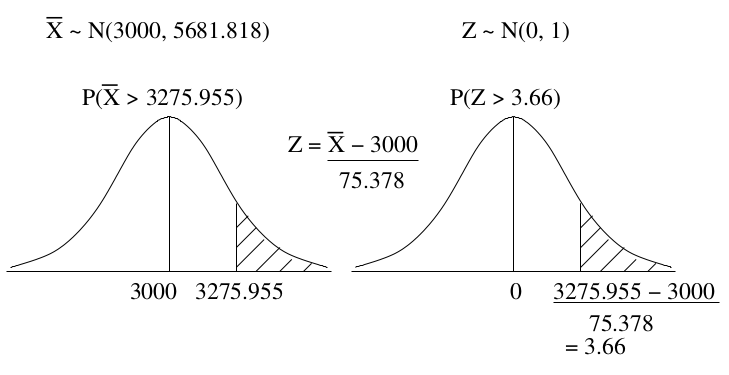
\includegraphics[scale=0.43]{pics/pvalue1.png}
	\caption{\cite{Marchini}}
\end{figure}




} 
\end{frame}


\begin{frame}{Example 2: Babies}
\scriptsize{

\begin{itemize}
 \item The probability we calculate is called the \textbf{p-value} of the test. 
 \item In this case the p-value is very low.
 \item This says that the probability of the data is very low if we assume the null hypothesis is true.
 \item But how low does this probability have to be before we can conclude that the null hypothesis is false.
 \item The convention within statistics is to choose a \textbf{level of significance} $\alpha$ before the experiment that dictates how low the p-value should be before we reject the null hypothesis. 
 \item In practice, many people use a significance level of 5\% and conclude that there is significant evidence against the null hypothesis if the p-value is less than or equal to 0.05.
 \item A more conservative approach uses a 1\% significance level and conclude that there is significant evidence against the null hypothesis if the p-value is less than 0.01.
 
\end{itemize}


} 
\end{frame}




\begin{frame}[fragile]{Example 2: Babies}
\scriptsize{

\begin{itemize}
 \item In our current example, the p-value is 0.00013 which is lower than $\alpha=0.05$. 
 \begin{verbatim}
> alpha<-0.05
> p.value<=alpha
[1] TRUE
 \end{verbatim}

 
 \item In this case, we would conclude that: \\ 
 ``there is significant evidence against the null hypothesis at the 5\% level''.
 \item Another way of saying this is that: \\
``we reject the null hypothesis at the 5\% level''
\item If the p-value for the test much larger, say 0.23, then we would conclude that: \\
``the evidence against the null hypothesis is not significant at the 5\% level''
\item Another way of saying this is that: \\
``we cannot reject the null hypothesis at the 5\% level''
  
\end{itemize}

} 
\end{frame}


\begin{frame}[fragile]{T-tests}
\scriptsize{

 \begin{itemize}
 \item In the previous example, we assumed that $\sigma$ was known.
 \item In many cases  $\sigma$ is unknown and we must estimate it using the unbiased estimator $s$ that we saw in the previous class.
 \item In these cases we can calculate a $T$ statistic $\frac{\overline{X_{n}}-\mu_{o}}{\frac{s}{\sqrt{n}}}$
 \begin{verbatim}
> s<-sd(babyboom$wt)
> s
[1] 528.0325
> se.t<-s/sqrt(n)
> se.t
[1] 79.60389
> 
> T.sta<-(xbar-mu0)/se.t
> T.sta
[1] 3.466596
 \end{verbatim}

 
\end{itemize}


} 
\end{frame}


\begin{frame}[fragile]{T-tests}
\scriptsize{

 \begin{itemize}
 \item From previous class we know that $T$ follows a t-student distribution with $n-1$ degrees of freedom  $T \sim t_{n-1}$.
 \item We can now  perform a T-test using the t-student distribution instead of a Gaussian.
 
 \item The p-value can be calculated analogously to the previous case now using the t-student distribution.
 
  
 \begin{verbatim}
> p.value<-1-pt(T.sta,df = n-1)
> p.value
[1] 0.0006042622
 \end{verbatim}

 \item We also reject the null hypothesis in this case with $\alpha=0.05$.
 \item But the p-value is larger than before.
 \item This is because the t-distribution has wider tails than the Normal distribution.
 \item The wide tails imply that there is more uncertainty because we had to estimate $\sigma$.
\end{itemize}


} 
\end{frame}


\begin{frame}[fragile]{T-tests}
\scriptsize{

 \begin{itemize}
 \item We can perform t-tests straightforwardly in R as follows:
 
 \begin{verbatim}
> t.test(x = babyboom$wt,mu = 3000, 
alternative = "greater",conf.level = 1-alpha)

	One Sample t-test

data:  babyboom$wt
t = 3.4666, df = 43, p-value = 0.0006043
alternative hypothesis: true mean is greater than 3000
95 percent confidence interval:
 3142.135      Inf
sample estimates:
mean of x 
 3275.955 
 \end{verbatim}

 
\end{itemize}


} 
\end{frame}


\begin{frame}[fragile]{Calculating a critical region}
\scriptsize{

 \begin{itemize}
 \item Another way of thinking about this test is that there is some critical region of values such that if the test statistic lies in this region then we will reject $H_0$.
 \item If the test statistic lies outside this region we will not reject $H_0$.
 \item In the babies example, using a 5\% level of significance this set of values will be the most extreme 5\% of values in the right hand tail of the distribution.
 \item We can calculate that the boundary of this region, called the critical value: 
 \begin{verbatim}
> crit<-qnorm(1-alpha)
> crit
[1] 1.644854
 \end{verbatim}

 
 \item The value of our test statistic is 3.66 which lies in the critical region so we reject the null hypothesis at the 5\% level.
  \begin{verbatim}
> Z.score>=crit
[1] TRUE
 \end{verbatim}

 
\end{itemize}


} 
\end{frame}


\begin{frame}[fragile]{Calculating a critical region}
\scriptsize{

 \begin{figure}[h!]
	\centering
	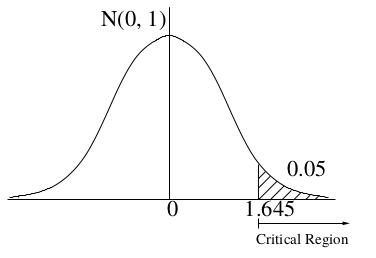
\includegraphics[scale=0.47]{pics/critregion.png}
\end{figure}


 \begin{itemize}
 \item Alternatively, using a T-distribution:
 \begin{verbatim}
 > crit2<-qt(1-alpha, df = n-1)
> crit2
[1] 1.681071
> T.sta>=crit2
[1] TRUE
 \end{verbatim}

 
\end{itemize}


} 
\end{frame}



\begin{frame}{Overview of NHST}
\scriptsize{
\begin{block}{The two hypotheses in NHST}
 \begin{itemize}
\scriptsize{
\item \textbf{Null Hypothesis} $H_{0}$: what has been considered real up to the present or what would we expect the data to look like if there is no effect.
\begin{itemize}
\scriptsize{
 \item The null hypothesis always involves some kind of equality ($=$).}
\end{itemize}



\item \textbf{Alternative Hypothesis} $H_{a}$: it is the alternative model that we want to consider or  what we expect if there actually is an effect. 
\begin{itemize}
\scriptsize{
 \item The alternative hypothesis always involves some kind of inequality ($\neq$, $>$, or $<$).}
\end{itemize}


}
 \end{itemize}
 
\end{block}


\begin{itemize}
\item Importantly, null hypothesis testing operates under the assumption that the null hypothesis is true unless the evidence shows otherwise.
\item The idea is to find enough \textbf{statistical evidence} to reject $H_{0}$ and be able to conclude $H_{a}$.
\item If we do not get enough statistical evidence \textbf{we fail to reject} $H_{0}$.
\end{itemize}



} 
\end{frame}



\begin{frame}{Overview of NHST}
\scriptsize{


\begin{block}{Methodology to Perform a Hypothesis Test}
\begin{itemize}
 \item Specify a null hypothesis $H_0$ and alternative $H_a$.
 \item Set a test significance level $\alpha$.
 \item Collect some data relevant to the hypothesis.
 \item Fit a model to the data and compute a test statistic $T$.
 \begin{itemize}
 \scriptsize{
 \item  In parametric tests, $T$ is a standardized value that (e.g., a Z-score).}
 \end{itemize}
 \item Assess the ``statistical significance'' of $T$.
\end{itemize}
\end{block}

The last part can be done with two approaches
\begin{itemize}
 \item P-value approach: compute the probability of the observed value (or more extreme values) of that statistic assuming that the null hypothesis is true and compare it with $\alpha$.

\item Critical region: Calculate a region of values such that if $T$ lies in this region then we will reject $H_0$ 

\end{itemize}



} 
\end{frame}



\begin{frame}{More on P-values}
\scriptsize{


\begin{itemize}
 \item Generally, in addition to knowing whether we reject or fail to reject a null hypothesis we want to quantify the evidence we have against it.
 \item P-values allow us to quantity this.
 
 \item A p-value is defined as the probability of obtaining an outcome \textbf{at least as extreme} as that observed in the data given that the null hypothesis is true.
 \item ``Extreme'' means far from the null hypothesis and favorable for the alternative hypothesis (larger than the sample mean in previous example).
 
 \item  We must consider all more extreme values because  the probability of any particular value (such as the observed sample mean) is zero for continuous distributions. 
 \item We must recall that we are trying to determine how weird our result would be if the null hypothesis were true.
 \item Hence, any result that is more extreme will be even more weird.
 \item So we want to count all of those weirder possibilities when we compute the probability of our result under the null hypothesis.
  
\end{itemize}



} 
\end{frame}



\begin{frame}[fragile]{Two-sided Tests}
\scriptsize{
\begin{itemize}
 \item In the previous example we wanted to test the research hypothesis that mean birth weight of Australian babies was greater than 3000g.
 \item This suggests that we had some prior information that the mean birth weight of Australian babies was definitely not lower than 3000g. 
 \item If this were not the case then our research hypothesis would be that the mean birth weight of Australian babies was different from 3000g. 
 \item This allows for the possibility that the mean birth weight could be less than or greater than 3000g.
 \item This is an example of a \textbf{two-sided} test as opposed to the previous example which was a \textbf{one-sided} test.
 
 \item In this two-sided case we would write our hypotheses as
 \begin{table}
\center
 \begin{tabular}{c}  
$H_0$: $\mu=3000g$ \\
$H_1$: $\mu\neq3000g$
\end{tabular} 
\end{table}
\end{itemize}
} 
\end{frame}



\begin{frame}[fragile]{Two-sided Tests}
\scriptsize{
\begin{itemize}
\item As before we would calculate our test statistic as 3.66 for the Normal distribution and 3.47 for the T-student. 
\item In this case we allow for the possibility that the mean value is less than 3000g by setting our critical region
to be lowest 2.5\% and highest 2.5\% of the distribution.
\item In this way the total area of the critical region remains 0.05 and so the level of significance $\alpha$ of our test remains 5\%. 
\item The critical values for a Z-test are:
\begin{verbatim}
> crit.left<-qnorm(alpha/2)
> crit.left
[1] -1.959964
> crit.right<-qnorm(1-alpha/2)
> crit.right
[1] 1.959964 
\end{verbatim}


\item Thus if our test
statistic is less than -1.96 or greater than 1.96 we would reject the null hypothesis.
\item In this example, the value of test statistic does lie in the critical region so we reject the null hypothesis at the 5\% level.
\begin{verbatim}
> Z.score<=crit.left | Z.score >= crit.right
[1] TRUE 
\end{verbatim}


\end{itemize}



} 
\end{frame}

\begin{frame}[fragile]{Two-sided Tests}
\scriptsize{

 \begin{figure}[h!]
	\centering
	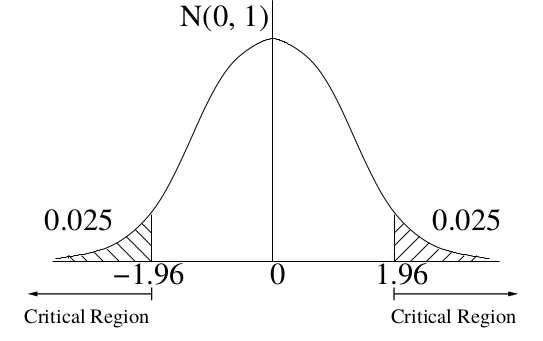
\includegraphics[scale=0.47]{pics/critregion2sided.png}
\end{figure}



} 
\end{frame}








\begin{frame}[fragile]{Two-sided Tests}
\scriptsize{
\begin{itemize}

\item For the case of the T-distribution our critical region is:
\begin{verbatim}
> crit2.left<-qt(alpha/2,df = n-1)
> crit2.left
[1] -2.016692
> crit2.right<-qt(1-alpha/2,df = n-1)
> crit2.right
[1] 2.016692
> 
> T.sta<=crit2.left |T.sta >= crit2.right
[1] TRUE
\end{verbatim}
\item Since $T$ is in the rejection region, we reject the null hypothesis.

\end{itemize}



} 
\end{frame}

\begin{frame}[fragile]{Two-sided Tests}
\scriptsize{
\begin{itemize}

\item Alternatively, we could calculate a confidence interval for the sample mean  with $(1-\alpha)\%$ confidence.

\item The confidence interval becomes the \textbf{acceptance region} and we reject $H_0$ if $\mu_0 =3000$ is not trapped by the interval.

\begin{verbatim}
> left.conf<-xbar-qt(p=1-alpha/2,n-1)*se.t
> left.conf
[1] 3115.418
> right.conf<-xbar+qt(p=1-alpha/2,n-1)*se.t
> right.conf
[1] 3436.491
> mu0 >= left.conf | mu0 <= right.conf
[1] TRUE
\end{verbatim}

\item Since  $\mu_0 =3000$ is not in my acceptance region, we reject the null hypothesis at the 0.05 significance level.

\item Confidence intervals and p-values always agree on statistical significance \cite{minitab_conf}. 

\end{itemize}



} 
\end{frame}



\begin{frame}[fragile]{Two-sided Tests}
\scriptsize{
\begin{itemize}

\item In order to calculate a p-value in a two-sided test we need to consider both left and right tails:

\begin{verbatim}
> pvalue<-pt(-T.sta,df=n-1)+(1-pt(T.sta,df=n-1))
> pvalue
[1] 0.001208524
> # or more compactly
> 2*pt(-abs(T.sta),df=n-1)
[1] 0.001208524
\end{verbatim}

\item Notice that this p-value is larger than for the one-sided test.

\item This reflects the fact that an extreme value is less surprising since it could have occurred in either direction.
\end{itemize}

} 
\end{frame}


\begin{frame}[fragile]{Two-sided Tests}
\scriptsize{
\begin{itemize}

\item We can run a two-sided t-test in R with one single call:
\end{itemize}

\begin{verbatim}
 > t.test(x=babyboom$wt,mu=3000,
 alternative="two.sided",conf.level = 1-alpha)

	One Sample t-test

data:  babyboom$wt
t = 3.4666, df = 43, p-value = 0.001209
alternative hypothesis: true mean is not equal to 3000
95 percent confidence interval:
 3115.418 3436.491
sample estimates:
mean of x 
 3275.955 
\end{verbatim}



} 
\end{frame}


\begin{frame}[fragile]{Unpaired Two Sample Tests}
 \scriptsize{

\begin{itemize}
 \item The babyboom dataset has a column specifying the gender of each baby.
 
 \begin{verbatim}
> summary(babyboom$gender)
girl  boy 
  18   26  
 \end{verbatim}

 
 \item Suppose our research hypothesis is that the mean birth weight of boys is different (two-sided) than mean birth weight of girls:

 \begin{table}
\center
 \begin{tabular}{c}  
$H_0$: $\mu_{boys}=\mu_{girls}$ or $\mu_{boys}-\mu_{girls}=0$  \\
$H_1$: $\mu_{boys}\neq\mu_{girls}$ or $\mu_{boys}-\mu_{girls}\neq0$
\end{tabular} 
\end{table}

\item We call this test a two sample tests (one sample with the births of boys and the other of girls).

\item The two samples are independent or unpaired (we have different number of observations for boys and girls).

\item This types of tests are very important for experimental data and observational studies (i.e., one sample is the control group and the other is the treatment).

 
\end{itemize}



}
\end{frame}



\begin{frame}[fragile]{Unpaired Two Sample Tests}
 \scriptsize{

\begin{itemize}
 
 \item Asymptotic theory tells us that the difference between two sample means (when the sample sizes are sufficiently large) has a Normal sampling distribution:
 
 \begin{displaymath}
  \overline{X}_{1}-\overline{X}_{2} \sim N\left(0, \frac{\sigma_1^{2}}{n_1} + \frac{\sigma_2^{2}}{n_2}\right)
 \end{displaymath}

  
 \item When the standard deviations of each group are unknown ($\sigma_1$, $\sigma_2$) we can estimate them as usual ($s_1$,$s_2$) and build the following $T$ satistics:
 
  \begin{displaymath}
  T = \frac{ \overline{X}_{1}-\overline{X}_{2}}{\sqrt{\frac{s_1^{2}}{n_1} + \frac{s_2^{2}}{n_2}}}
 \end{displaymath}

 \item The $T$ statistic is distributed according to a t-student distribution.
 
 
\end{itemize}



}
\end{frame}

\begin{frame}{Unpaired Two Sample Tests}
 \scriptsize{

\begin{itemize}
 
 \item When the groups are the same size and have equal variance, the degrees of freedom for the $T$ test is  $n_1+n_2-2$.
 
  \item In this case the box plot shows that the ``girl'' group is more variable than then ``boy'' group.
  
  \item We also know that the number of observations in each group is different.
 
 
  \begin{figure}[h!]
	\centering
	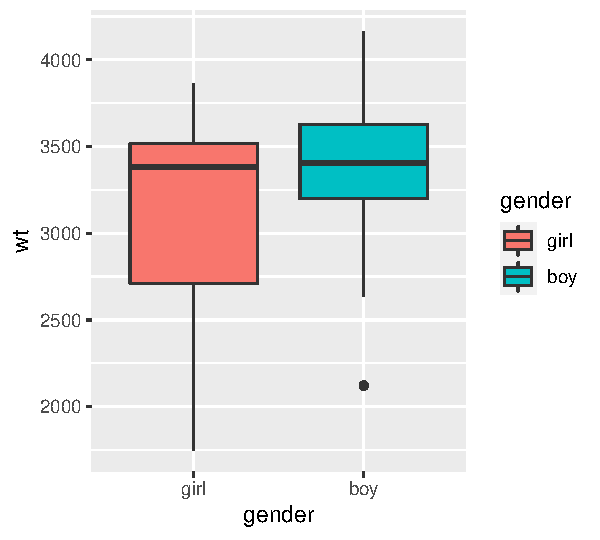
\includegraphics[scale=0.55]{pics/boxplotgender.pdf}
\end{figure}

 
\end{itemize}



}
\end{frame}


\begin{frame}{Unpaired Two Sample Tests}
 \scriptsize{

\begin{itemize}
 
 \item We need to use a more complex formula for the degrees of freedom, which is often referred to as a ``Welch t-test'':
 
 \begin{displaymath}
  d.f. = \frac{\left(\frac{s_1^{2}}{n_1} + \frac{s_2^{2}}{n_2}\right)^2}{\frac{(s_1^2/n_1)^2}{n_1-1}+\frac{(s_2^2/n_2)^2}{n_2-1}}
 \end{displaymath}

 
 
 \item For this example d.f. = 27.631 which is lower than what we would get by subtracting 2 from the sample size.
  
 
 \item Recall that the lower the d.f the wider the tails in the t-student distribution.
 
 \item This is essentially, imposing a penalty on the test for differences in sample size or variance.
 

 
 
\end{itemize}



}
\end{frame}

\begin{frame}[fragile]{Unpaired Two Sample Tests}
 \scriptsize{

\begin{itemize}
 
 \item We can run a Welsh T-test in R as follows:
 
 \begin{verbatim}
> t.test(babyboom$wt~babyboom$gender)

	Welch Two Sample t-test

data:  babyboom$wt by babyboom$gender
t = -1.4211, df = 27.631, p-value = 0.1665
alternative hypothesis: true difference in means is not equal to 0
95 percent confidence interval:
 -593.1538  107.4273
sample estimates:
mean in group girl  mean in group boy 
          3132.444           3375.308 
  
 \end{verbatim}

 
\item In this case, we fail to reject $H_0$ at the $5\%$ significance level.
 
 
\end{itemize}



}
\end{frame}



\begin{frame}{Paired Two Sample Tests}
 \scriptsize{

\begin{itemize}
 
 \item Another very useful type of two sample test is the Paired T-Test.
 \item This test is used to compare the means between two \textbf{related groups} of samples.
 \item Here we have two values (i.e., pair of values) for the same samples \cite{sthda}.
 \item This type of data arises when we compare a response variable after and before a treatment for each subject.
 \item It also arises in matched pairs experiments.
 
 \item Paired t-test analysis is performed as follow:

   \begin{enumerate}
   \scriptsize{
    \item Calculate the difference $d$ between each pair of value.
    \item Compute the mean $\overline{d}$ and the standard deviation $s_d$ of these differences.
    \item Compare the $\overline{d}$ to 0 in the same way as previous tests.}
   \end{enumerate}
 


\end{itemize}



}
\end{frame}



\begin{frame}{Paired Two Sample Tests}
 \scriptsize{

\begin{itemize}
 
 \item The test statistics $T$ is calculated as follows for the paired test:
 \begin{displaymath}
  T = \frac{\overline{d}}{s_d/\sqrt{n}}
 \end{displaymath}

 \item The the degrees of freedom (df) are simply $n-1$.

\item As an example of data, 20 mice received a treatment X during 3 months.

\item We want to know whether the treatment X has an impact on the weight of the mice.

\item The weight of the 20 mice has been measured before and after the treatment. 

\item Let's test the following hypotheses:
 
  \begin{table}
\center
 \begin{tabular}{c}  
$H_0$: $\overline{d}=0$  \\
$H_1$: $\overline{d}\neq0$
\end{tabular} 
\end{table}
 
\end{itemize}



}
\end{frame}

\begin{frame}[fragile]{Paired Two Sample Tests}
 \scriptsize{

\begin{itemize}
 
 \item We can run a paired t-test in R as follows:
 
 
\end{itemize}

\begin{verbatim}
> before <-c(200.1, 190.9, 192.7, 213, 241.4, 196.9, 172.2,
+            185.5, 205.2, 193.7)
> # Weight of the mice after treatment
> after <-c(392.9, 393.2, 345.1,393, 434, 427.9, 422, 
+           383.9, 392.3, 352.2)
> t.test(after, before, paired = TRUE, alternative = "two.sided")

	Paired t-test

data:  after and before
t = 20.883, df = 9, p-value = 6.2e-09
alternative hypothesis: true difference in means is not equal to 0
95 percent confidence interval:
 173.4219 215.5581
sample estimates:
mean of the differences 
                 194.49 
\end{verbatim}


}
\end{frame}





\begin{frame}{Errors}
 \scriptsize{

\begin{itemize}
 \item We have two types of errors when we perform a hypothesis test
 \item Type I error: it is when we reject the null hypothesis when it was true (also called ``false alarm'').
  \item Type II error: is when the null hypothesis is false but we do not have statistical evidence to reject it (also called a ``miss'').
  
   \begin{table}
\begin{tabular}{c | c c}
\hline
  & Retain $H_0$ &  Reject $H_{0}$   \\ 
\hline
$H_0$ true & \checkmark & type I error \\
$H_1$ true & type II error & \checkmark \\
\hline
\end{tabular}
\end{table}
  
\item Neyman and Pearson coined two terms to describe the probability of these two types of errors in the long run:

\begin{itemize}
\scriptsize{
 \item $P$(Type I error) = $\alpha$
  \item $P$(Type II error) = $\beta$}
\end{itemize}
\end{itemize}



}
\end{frame}


\begin{frame}{Errors}
 \scriptsize{

\begin{itemize}
 \item If we set $\alpha$ to .05, then in the long run we should make a Type I error 5\% of the time. 
 \item The standard value for an acceptable level of $\beta$ is .2.
 \item That is, we are willing to accept that 20\% of the time we will fail to detect a true effect when it truly exists.
  \item The concept of \textbf{statistical power} is the complement of Type II error: 
  \begin{displaymath}                                                                               
 power = 1 - \beta                                                                                      \end{displaymath}

  
 \item The power of a test is the likelihood of finding a positive result given that it exists.\cite{poldrack2019statistical}
 
 \item To mitigate type I errors we generally use smaller values of $\alpha$.
 \item To mitigate type II errors (or increase the power of the test) we generally work with larger samples.
 \item There is a trade-off between type I and type II errors. 
 \item There are tools to analyze the power of a test that go beyond the scope of this course.
\end{itemize}



}
\end{frame}






\begin{frame}{What does a significant result mean?}
\scriptsize{
\begin{itemize}
 \item There is a great deal of confusion about what p-values actually mean.
 \item Suppose we do an experiment comparing the means between conditions, and we find a difference with a p-value of .01.
 \item Does it mean that the probability of the null hypothesis being true is .01?
 \begin{itemize}
 \scriptsize{
  \item No. Remember that in NHST, the p-value is the probability of the data given the null hypothesis: $P(data|H_0)$.
  \item It does not warrant conclusions about the probability of the null hypothesis given the data: $P(H_0|data)$. }
 \end{itemize}
\item  Does it mean that the probability that you are making the wrong decision is .01? 
\begin{itemize}
\scriptsize{
 \item No. This would be $P(H_0|data)$, but remember as above that p-values are probabilities of data under $H_0$, not probabilities of hypotheses.}
\end{itemize}

 
 
\end{itemize}
}
 
\end{frame}



\begin{frame}{What does a significant result mean?}
\scriptsize{
\begin{itemize}

 \item  Does it mean that you have found a practically important effect?
 \begin{itemize}
 \scriptsize{
  \item No. There is an essential distinction between statistical significance and practical significance. 
  \item Suppose we performed an RCT to examine the effect of a particular diet on body weight, and we find a statistically significant effect at $p<.05$. 
  \item This doesn't tell us how much weight was actually lost.
  \item The loss of one ounce (i.e. the weight of a few potato chips) can be statistically significant but not practically significant.
  
  }
 \end{itemize}
\item  Many scientist think that NHST is flawed and that is has been the cause of serious problems in science \cite{poldrack2019statistical}.

 \item For example, The American Statistical Association (ASA) released a ``Statement on Statistical Significance and P-Values'' indicating the proper use and interpretation of the p-value \cite{wasserstein2016asa}.
 
\end{itemize}
}
 
\end{frame}


\begin{frame}{There are many other tests}
 \scriptsize{
There are a plethora of other tests that we will not teach in this course
 
\begin{itemize}
 \item Proportion tests.
 \item The Fisher's exact test.
 \item Analysis of Variance (ANOVA).
 \item The Chi-square tests of independence.
 \item The Wilcoxon signed-rank test.
 \item The Kolmogorov–Smirnov tests. 
 
\end{itemize}


}
\end{frame}


\begin{frame}{Conclusions}
 \scriptsize{

\begin{itemize}
 \item  In this class we have introduced two important statistical concepts: design of experiments and NHST.  
 \item Experiments are a powerful approach to determining cause-effect relationships.
 \item It is very important to identify and control confounding variables in the design of experiments.
 \item Hypothesis testing is a family of techniques for testing hypotheses using data.
 \item NHST must be used with care and we should always remind that p-values do not measure the probability of a given hypothesis.
\end{itemize}


}
\end{frame}




%%%%%%%%%%%%%%%%%%%%%%%%%%%
%%%%%%%%%%%%%%%%%%%%%%%%%%%
\begin{frame}[allowframebreaks]\scriptsize
\frametitle{References}
\bibliography{bio}
\bibliographystyle{apalike}
%\bibliographystyle{flexbib}
\end{frame}  









%%%%%%%%%%%%%%%%%%%%%%%%%%%

\end{document}
